% vi:ft=tex
\documentclass{standalone}

\usepackage{tikz}
\usepackage{verbatim}

\usetikzlibrary{arrows}
\usetikzlibrary{calc}

\begin{document}

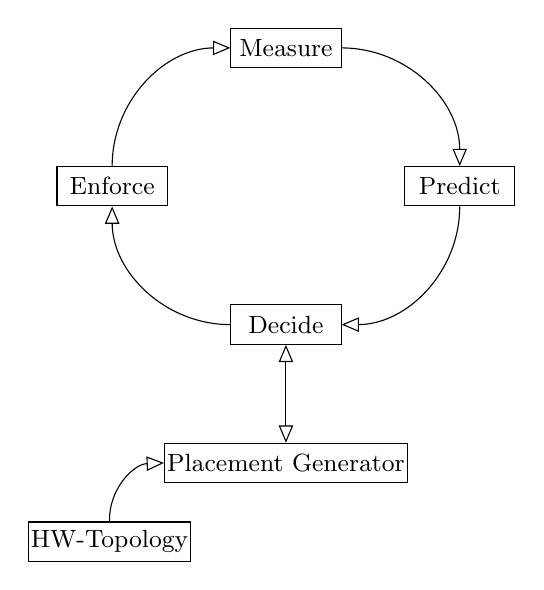
\begin{tikzpicture}[node distance=1.5cm]

  % Colors
  % Styles
  \tikzstyle{defaultRec} = [font=\small, text centered, inner sep = 1pt,
    draw=black, shape=rectangle, fill=white, minimum height = .5cm, minimum
  width = 1.4cm];

  \tikzstyle{arrow} = [-open triangle 45, black];

  % Variables
  \newcommand\Ymax{3};
  \newcommand\Xmax{7};
  \newcommand\fstLvl{1};
  \newcommand\sndLvl{2};

  % Drawing

%  \foreach \x in {-3,-2.5,...,3}
%    \draw[black,very thin] (\x cm,-5cm) -- (\x cm,3cm);
%
%  \foreach \y in {-5,-4.5,...,3}
%    \draw[black,very thin] (-3cm,\y cm) -- (3cm,\y cm);

  \node(center) [] {};

  \node(meas) [defaultRec, above of=center, anchor=south] {Measure};
  \node(pred) [defaultRec, right of=center, anchor=west] {Predict};
  \node(deci) [defaultRec, below of=center, anchor=north] {Decide};
  \node(enf)  [defaultRec, left of=center, anchor=east] {Enforce};
  \node(place) [defaultRec, below of=deci, anchor=north] {Placement Generator};

  \node(help) [node distance=1cm,below of=place] {};
  \node(topo) [defaultRec, left of=help, anchor=east,xshift=3mm] {HW-Topology};

  \draw[arrow] (meas.east) to [bend left=45] (pred.north);
  \draw[arrow] (pred.south) to [bend left=45] (deci.east);
  \draw[arrow] (deci.west) to [bend left=45] (enf.south);
  \draw[arrow] (enf.north) to [bend left=45] (meas.west);
  \draw[open triangle 45 - open triangle 45, black] (deci.south) -- (place.north);
%  \draw[arrow] (topo.north) .. controls +(up:12mm) and +(left:10mm)
%				 .. (place.west);

  \draw[arrow] (topo.north) to [bend left=45] (place.west);
%  \draw[arrow,blue] (pred.south) to [bend left=45] (deci.east);

\end{tikzpicture}

\end{document}
